% Options for packages loaded elsewhere
\PassOptionsToPackage{unicode}{hyperref}
\PassOptionsToPackage{hyphens}{url}
%
\documentclass[
]{article}
\usepackage{lmodern}
\usepackage{amsmath}
\usepackage{ifxetex,ifluatex}
\ifnum 0\ifxetex 1\fi\ifluatex 1\fi=0 % if pdftex
  \usepackage[T1]{fontenc}
  \usepackage[utf8]{inputenc}
  \usepackage{textcomp} % provide euro and other symbols
  \usepackage{amssymb}
\else % if luatex or xetex
  \usepackage{unicode-math}
  \defaultfontfeatures{Scale=MatchLowercase}
  \defaultfontfeatures[\rmfamily]{Ligatures=TeX,Scale=1}
\fi
% Use upquote if available, for straight quotes in verbatim environments
\IfFileExists{upquote.sty}{\usepackage{upquote}}{}
\IfFileExists{microtype.sty}{% use microtype if available
  \usepackage[]{microtype}
  \UseMicrotypeSet[protrusion]{basicmath} % disable protrusion for tt fonts
}{}
\makeatletter
\@ifundefined{KOMAClassName}{% if non-KOMA class
  \IfFileExists{parskip.sty}{%
    \usepackage{parskip}
  }{% else
    \setlength{\parindent}{0pt}
    \setlength{\parskip}{6pt plus 2pt minus 1pt}}
}{% if KOMA class
  \KOMAoptions{parskip=half}}
\makeatother
\usepackage{xcolor}
\IfFileExists{xurl.sty}{\usepackage{xurl}}{} % add URL line breaks if available
\IfFileExists{bookmark.sty}{\usepackage{bookmark}}{\usepackage{hyperref}}
\hypersetup{
  pdftitle={DA3 Assignment 1},
  hidelinks,
  pdfcreator={LaTeX via pandoc}}
\urlstyle{same} % disable monospaced font for URLs
\usepackage[margin=1in]{geometry}
\usepackage{graphicx}
\makeatletter
\def\maxwidth{\ifdim\Gin@nat@width>\linewidth\linewidth\else\Gin@nat@width\fi}
\def\maxheight{\ifdim\Gin@nat@height>\textheight\textheight\else\Gin@nat@height\fi}
\makeatother
% Scale images if necessary, so that they will not overflow the page
% margins by default, and it is still possible to overwrite the defaults
% using explicit options in \includegraphics[width, height, ...]{}
\setkeys{Gin}{width=\maxwidth,height=\maxheight,keepaspectratio}
% Set default figure placement to htbp
\makeatletter
\def\fps@figure{htbp}
\makeatother
\setlength{\emergencystretch}{3em} % prevent overfull lines
\providecommand{\tightlist}{%
  \setlength{\itemsep}{0pt}\setlength{\parskip}{0pt}}
\setcounter{secnumdepth}{-\maxdimen} % remove section numbering
\usepackage{booktabs}
\usepackage{longtable}
\usepackage{array}
\usepackage{multirow}
\usepackage{wrapfig}
\usepackage{float}
\usepackage{colortbl}
\usepackage{pdflscape}
\usepackage{tabu}
\usepackage{threeparttable}
\usepackage{threeparttablex}
\usepackage[normalem]{ulem}
\usepackage{makecell}
\usepackage{xcolor}
\usepackage{caption}
\usepackage{graphicx}
\usepackage{siunitx}
\usepackage{ulem}
\usepackage{hhline}
\usepackage{calc}
\usepackage{tabularx}
\usepackage{adjustbox}
\usepackage{hyperref}
\ifluatex
  \usepackage{selnolig}  % disable illegal ligatures
\fi

\title{DA3 Assignment 1}
\usepackage{etoolbox}
\makeatletter
\providecommand{\subtitle}[1]{% add subtitle to \maketitle
  \apptocmd{\@title}{\par {\large #1 \par}}{}{}
}
\makeatother
\subtitle{Airbnb prediction models: New York}
\author{}
\date{\vspace{-2.5em}}

\begin{document}
\maketitle

\hypertarget{introduction}{%
\subsection{Introduction}\label{introduction}}

This is a report for Data Analysis 3: Assignment 1. The task is to
perform prediction using the knowledge we obtained in the course.

As a first step, we define a business question: to help a company
operating small and mid-size apartments hosting 2-6 guests. The company
is set to price their new apartments not on the market. For this, I
built a price prediction model similarly to how we did in our case study
for London (Hackney borough). Also, discussion of my modeling decisions
and comparison of my results is provided at the end. In the next step, I
define the data for analysis (sample design). For this, I obtained data
from \href{http://insideairbnb.com/get-the-data.html}{insideairbnb.com}
website. Data is for New York, it was compiled on 10 December, 2020.

\hypertarget{label-engineering}{%
\subsection{Label Engineering}\label{label-engineering}}

We have a quantitative y - price in USD dollars. That's why I leave y as
it is (without any transformation).

\hypertarget{feature-engineering}{%
\subsection{Feature engineering}\label{feature-engineering}}

\hypertarget{data-cleaning}{%
\subsubsection{Data cleaning}\label{data-cleaning}}

The original dataset that was obtained from the website contained 36923
rows and 62 columns. I decided to remove several columns that are not
used in the analysis (see Appendix).

Then dollar signs (``\$'') were removed from price column. Also, false
(f) and true (t) values were replaced with 1 and 0.

Amenities column consisted of several values. These values in the row
were pivoted as a column of dummy variable. List of amenities is given
in Appendix.

Code for data cleaning is provided in \textbf{data-cleaning-NY.R} file.

\hypertarget{data-preparation}{%
\subsubsection{Data preparation}\label{data-preparation}}

When dataset was inspected, it was clear that ``Entire apartment'',
``Private room in apartment'', and ``Entire condominium'' were the most
frequent property type (Appendix). Therefore, I decided to filter out
the dataset and leave only observations that have these property types.

Dummy variables were created from amenities column (that starts with
`d'). I kept dummy variables, numerical and factorial (categorical)
columns and removed all other columns that are not used for the
analysis. After that, I left with 49 columns (variables).

The observations where the value for price column is missing were
dropped as our analysis will be prediction of price.

I decided to narrow down my focus and filtered dataset so that it
includes observations only from Manhattan neighborhood. After that,
28402 observations decreased to 14170.

\hypertarget{exploratory-data-analysis}{%
\subsubsection{Exploratory data
analysis}\label{exploratory-data-analysis}}

We can see that minimum price is 10 dollars and maximum price is 999
dollars. Average price is 152.1 dollars.

 
  \providecommand{\huxb}[2]{\arrayrulecolor[RGB]{#1}\global\arrayrulewidth=#2pt}
  \providecommand{\huxvb}[2]{\color[RGB]{#1}\vrule width #2pt}
  \providecommand{\huxtpad}[1]{\rule{0pt}{#1}}
  \providecommand{\huxbpad}[1]{\rule[-#1]{0pt}{#1}}

\begin{table}[ht]
\begin{centerbox}
\begin{threeparttable}
\captionsetup{justification=centering,singlelinecheck=off}
\caption{Summary of prices}
 \label{tab:unnamed-chunk-4}
\setlength{\tabcolsep}{0pt}
\begin{tabular}{l l l l l l l l l l l l}


\hhline{}
\arrayrulecolor{black}

\multicolumn{1}{!{\huxvb{0, 0, 0}{0}}r!{\huxvb{0, 0, 0}{0}}}{\huxtpad{6pt + 1em}\raggedleft \hspace{6pt}  \hspace{6pt}\huxbpad{6pt}} &
\multicolumn{1}{l!{\huxvb{0, 0, 0}{0}}}{\huxtpad{6pt + 1em}\raggedright \hspace{6pt} V1 \hspace{6pt}\huxbpad{6pt}} &
\multicolumn{1}{r!{\huxvb{0, 0, 0}{0}}}{\huxtpad{6pt + 1em}\raggedleft \hspace{6pt}  \hspace{6pt}\huxbpad{6pt}} &
\multicolumn{1}{l!{\huxvb{0, 0, 0}{0}}}{\huxtpad{6pt + 1em}\raggedright \hspace{6pt} V1 \hspace{6pt}\huxbpad{6pt}} &
\multicolumn{1}{r!{\huxvb{0, 0, 0}{0}}}{\huxtpad{6pt + 1em}\raggedleft \hspace{6pt}  \hspace{6pt}\huxbpad{6pt}} &
\multicolumn{1}{l!{\huxvb{0, 0, 0}{0}}}{\huxtpad{6pt + 1em}\raggedright \hspace{6pt} V1 \hspace{6pt}\huxbpad{6pt}} &
\multicolumn{1}{r!{\huxvb{0, 0, 0}{0}}}{\huxtpad{6pt + 1em}\raggedleft \hspace{6pt}  \hspace{6pt}\huxbpad{6pt}} &
\multicolumn{1}{l!{\huxvb{0, 0, 0}{0}}}{\huxtpad{6pt + 1em}\raggedright \hspace{6pt} V1 \hspace{6pt}\huxbpad{6pt}} &
\multicolumn{1}{r!{\huxvb{0, 0, 0}{0}}}{\huxtpad{6pt + 1em}\raggedleft \hspace{6pt}  \hspace{6pt}\huxbpad{6pt}} &
\multicolumn{1}{l!{\huxvb{0, 0, 0}{0}}}{\huxtpad{6pt + 1em}\raggedright \hspace{6pt} V1 \hspace{6pt}\huxbpad{6pt}} &
\multicolumn{1}{r!{\huxvb{0, 0, 0}{0}}}{\huxtpad{6pt + 1em}\raggedleft \hspace{6pt}  \hspace{6pt}\huxbpad{6pt}} &
\multicolumn{1}{l!{\huxvb{0, 0, 0}{0}}}{\huxtpad{6pt + 1em}\raggedright \hspace{6pt} V1 \hspace{6pt}\huxbpad{6pt}} \tabularnewline[-0.5pt]


\hhline{}
\arrayrulecolor{black}

\multicolumn{1}{!{\huxvb{0, 0, 0}{0}}r!{\huxvb{0, 0, 0}{0}}}{\huxtpad{6pt + 1em}\raggedleft \hspace{6pt} Min. \hspace{6pt}\huxbpad{6pt}} &
\multicolumn{1}{l!{\huxvb{0, 0, 0}{0}}}{\huxtpad{6pt + 1em}\raggedright \hspace{6pt} 10 \hspace{6pt}\huxbpad{6pt}} &
\multicolumn{1}{r!{\huxvb{0, 0, 0}{0}}}{\huxtpad{6pt + 1em}\raggedleft \hspace{6pt} 1st Qu. \hspace{6pt}\huxbpad{6pt}} &
\multicolumn{1}{l!{\huxvb{0, 0, 0}{0}}}{\huxtpad{6pt + 1em}\raggedright \hspace{6pt} 80 \hspace{6pt}\huxbpad{6pt}} &
\multicolumn{1}{r!{\huxvb{0, 0, 0}{0}}}{\huxtpad{6pt + 1em}\raggedleft \hspace{6pt} Median \hspace{6pt}\huxbpad{6pt}} &
\multicolumn{1}{l!{\huxvb{0, 0, 0}{0}}}{\huxtpad{6pt + 1em}\raggedright \hspace{6pt} 120 \hspace{6pt}\huxbpad{6pt}} &
\multicolumn{1}{r!{\huxvb{0, 0, 0}{0}}}{\huxtpad{6pt + 1em}\raggedleft \hspace{6pt} Mean \hspace{6pt}\huxbpad{6pt}} &
\multicolumn{1}{l!{\huxvb{0, 0, 0}{0}}}{\huxtpad{6pt + 1em}\raggedright \hspace{6pt} 152 \hspace{6pt}\huxbpad{6pt}} &
\multicolumn{1}{r!{\huxvb{0, 0, 0}{0}}}{\huxtpad{6pt + 1em}\raggedleft \hspace{6pt} 3rd Qu. \hspace{6pt}\huxbpad{6pt}} &
\multicolumn{1}{l!{\huxvb{0, 0, 0}{0}}}{\huxtpad{6pt + 1em}\raggedright \hspace{6pt} 186 \hspace{6pt}\huxbpad{6pt}} &
\multicolumn{1}{r!{\huxvb{0, 0, 0}{0}}}{\huxtpad{6pt + 1em}\raggedleft \hspace{6pt} Max. \hspace{6pt}\huxbpad{6pt}} &
\multicolumn{1}{l!{\huxvb{0, 0, 0}{0}}}{\huxtpad{6pt + 1em}\raggedright \hspace{6pt} 999 \hspace{6pt}\huxbpad{6pt}} \tabularnewline[-0.5pt]


\hhline{}
\arrayrulecolor{black}
\end{tabular}
\end{threeparttable}\par\end{centerbox}

\end{table}
 

The distribution price shown below. The price is normally distributed,
most of the observations having a price between 10 and 250. The plot is
skewed to the right indicating some of the extreme values on the right
tail (expensive apartments).

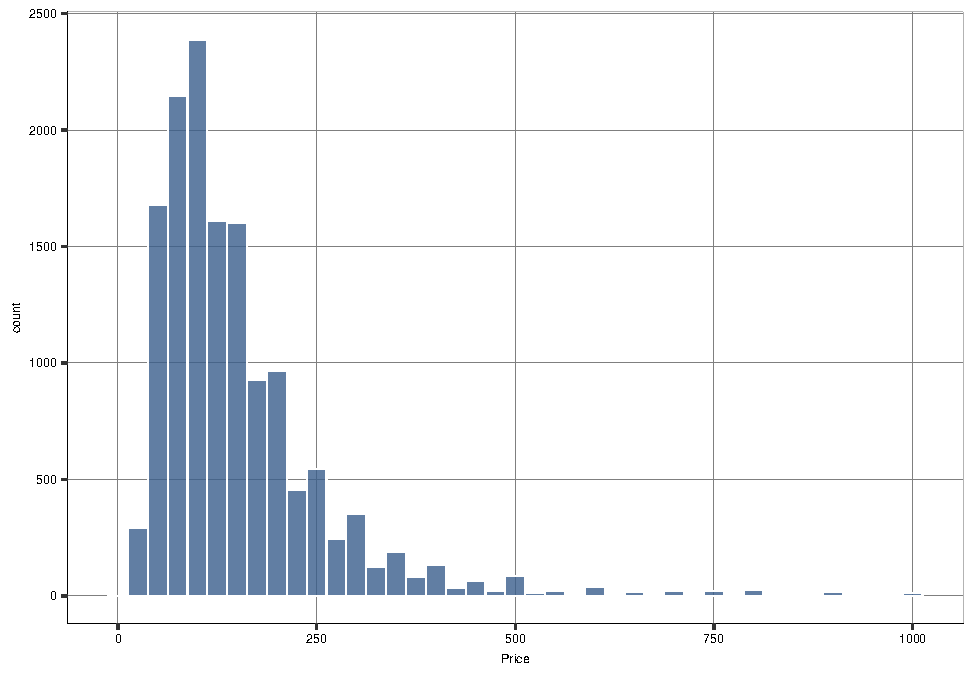
\includegraphics{report_files/figure-latex/unnamed-chunk-5-1.pdf}

\hypertarget{missing-values}{%
\subsubsection{Missing values}\label{missing-values}}

I checked in which columns there are missing values. For the columns
with few missing values, I imputed values as they don't have big
importance. The columns inlude beds, bathrooms, minimum\_nights,
number\_of\_reviews.

For the columns that are related to reviews, I replaced missing values
(reviews) with zero when there is no review and I added flags (1 if
replaced).

Currently, there are 8675 observations that are Entire apartments, 561
Entire condominiums and 4934 observations that are ``Private room in
apartment''.

As we are interested in the price of apartments that can accomodate 2-6
people, I used filter so that dataset contains apartments which
accommodate 2-6 people.

Code for data preparation is provided in \textbf{data-prepare-NY.R}
file.

\hypertarget{functional-form}{%
\subsubsection{Functional Form}\label{functional-form}}

To decide what functional form to use for the models, I checked
interactions between variables.

 
  \providecommand{\huxb}[2]{\arrayrulecolor[RGB]{#1}\global\arrayrulewidth=#2pt}
  \providecommand{\huxvb}[2]{\color[RGB]{#1}\vrule width #2pt}
  \providecommand{\huxtpad}[1]{\rule{0pt}{#1}}
  \providecommand{\huxbpad}[1]{\rule[-#1]{0pt}{#1}}

\begin{table}[ht]
\begin{centerbox}
\begin{threeparttable}
\captionsetup{justification=centering,singlelinecheck=off}
\caption{Average price by property_type, room_type}
 \label{tab:unnamed-chunk-6}
\setlength{\tabcolsep}{0pt}
\begin{tabular}{l l l}


\hhline{}
\arrayrulecolor{black}

\multicolumn{1}{!{\huxvb{0, 0, 0}{0}}l!{\huxvb{0, 0, 0}{0}}}{\huxtpad{6pt + 1em}\raggedright \hspace{6pt} f\_property\_type \hspace{6pt}\huxbpad{6pt}} &
\multicolumn{1}{l!{\huxvb{0, 0, 0}{0}}}{\huxtpad{6pt + 1em}\raggedright \hspace{6pt} f\_room\_type \hspace{6pt}\huxbpad{6pt}} &
\multicolumn{1}{r!{\huxvb{0, 0, 0}{0}}}{\huxtpad{6pt + 1em}\raggedleft \hspace{6pt} mean\_price \hspace{6pt}\huxbpad{6pt}} \tabularnewline[-0.5pt]


\hhline{}
\arrayrulecolor{black}

\multicolumn{1}{!{\huxvb{0, 0, 0}{0}}l!{\huxvb{0, 0, 0}{0}}}{\huxtpad{6pt + 1em}\raggedright \hspace{6pt} Entire apartment \hspace{6pt}\huxbpad{6pt}} &
\multicolumn{1}{l!{\huxvb{0, 0, 0}{0}}}{\huxtpad{6pt + 1em}\raggedright \hspace{6pt} Entire home/apt \hspace{6pt}\huxbpad{6pt}} &
\multicolumn{1}{r!{\huxvb{0, 0, 0}{0}}}{\huxtpad{6pt + 1em}\raggedleft \hspace{6pt} 177~~ \hspace{6pt}\huxbpad{6pt}} \tabularnewline[-0.5pt]


\hhline{}
\arrayrulecolor{black}

\multicolumn{1}{!{\huxvb{0, 0, 0}{0}}l!{\huxvb{0, 0, 0}{0}}}{\huxtpad{6pt + 1em}\raggedright \hspace{6pt} Entire condominium \hspace{6pt}\huxbpad{6pt}} &
\multicolumn{1}{l!{\huxvb{0, 0, 0}{0}}}{\huxtpad{6pt + 1em}\raggedright \hspace{6pt} Entire home/apt \hspace{6pt}\huxbpad{6pt}} &
\multicolumn{1}{r!{\huxvb{0, 0, 0}{0}}}{\huxtpad{6pt + 1em}\raggedleft \hspace{6pt} 249~~ \hspace{6pt}\huxbpad{6pt}} \tabularnewline[-0.5pt]


\hhline{}
\arrayrulecolor{black}

\multicolumn{1}{!{\huxvb{0, 0, 0}{0}}l!{\huxvb{0, 0, 0}{0}}}{\huxtpad{6pt + 1em}\raggedright \hspace{6pt} Private room in apartment \hspace{6pt}\huxbpad{6pt}} &
\multicolumn{1}{l!{\huxvb{0, 0, 0}{0}}}{\huxtpad{6pt + 1em}\raggedright \hspace{6pt} Private room \hspace{6pt}\huxbpad{6pt}} &
\multicolumn{1}{r!{\huxvb{0, 0, 0}{0}}}{\huxtpad{6pt + 1em}\raggedleft \hspace{6pt} 94.6 \hspace{6pt}\huxbpad{6pt}} \tabularnewline[-0.5pt]


\hhline{}
\arrayrulecolor{black}
\end{tabular}
\end{threeparttable}\par\end{centerbox}

\end{table}
 

\hypertarget{appendix}{%
\subsection{Appendix}\label{appendix}}

\hypertarget{data-cleaning-1}{%
\subsubsection{Data Cleaning}\label{data-cleaning-1}}

Removed columns:

``host\_thumbnail\_url'',``host\_picture\_url'',``listing\_url'',``thumbnail\_url'',``medium\_url'',``picture\_url'',``xl\_picture\_url'',``host\_url'',``last\_scraped'',``description'',
``experiences\_offered'', ``neighborhood\_overview'', ``notes'',
``transit'', ``access'', ``interaction'', ``house\_rules'',
``host\_about'', ``host\_response\_time'', ``name'', ``summary'',
``space'', ``host\_location''

Amenities:

``conditioner'', ``stove'', ``hdtv'', ``tv'', ``conditioning'', ``sound
system'', ``refrigerator'', ``shampoo'', ``soap'', ``oven'',
``toiletries'', ``speaker'', ``fan'', ``heating'', ``breakfast'',
``table'', ``dishwasher'', ``dryer'', ``elevator'', ``fitness'',
``parking'', ``garage'', ``wifi'', ``game'', ``garden'', ``gym'',
``restaurant'', ``bar'', ``washer'', ``barbeque'', ``bbq''

Property types:

 
  \providecommand{\huxb}[2]{\arrayrulecolor[RGB]{#1}\global\arrayrulewidth=#2pt}
  \providecommand{\huxvb}[2]{\color[RGB]{#1}\vrule width #2pt}
  \providecommand{\huxtpad}[1]{\rule{0pt}{#1}}
  \providecommand{\huxbpad}[1]{\rule[-#1]{0pt}{#1}}

\begin{table}[ht]
\begin{centerbox}
\begin{threeparttable}
\captionsetup{justification=centering,singlelinecheck=off}
\caption{Property types}
 \label{tab:unnamed-chunk-7}
\setlength{\tabcolsep}{0pt}
\begin{tabular}{l l}


\hhline{}
\arrayrulecolor{black}

\multicolumn{1}{!{\huxvb{0, 0, 0}{0}}r!{\huxvb{0, 0, 0}{0}}}{\huxtpad{6pt + 1em}\raggedleft \hspace{6pt}  \hspace{6pt}\huxbpad{6pt}} &
\multicolumn{1}{l!{\huxvb{0, 0, 0}{0}}}{\huxtpad{6pt + 1em}\raggedright \hspace{6pt} V1 \hspace{6pt}\huxbpad{6pt}} \tabularnewline[-0.5pt]


\hhline{}
\arrayrulecolor{black}

\multicolumn{1}{!{\huxvb{0, 0, 0}{0}}r!{\huxvb{0, 0, 0}{0}}}{\huxtpad{6pt + 1em}\raggedleft \hspace{6pt} Entire apartment \hspace{6pt}\huxbpad{6pt}} &
\multicolumn{1}{l!{\huxvb{0, 0, 0}{0}}}{\huxtpad{6pt + 1em}\raggedright \hspace{6pt} 15577 \hspace{6pt}\huxbpad{6pt}} \tabularnewline[-0.5pt]


\hhline{}
\arrayrulecolor{black}

\multicolumn{1}{!{\huxvb{0, 0, 0}{0}}r!{\huxvb{0, 0, 0}{0}}}{\huxtpad{6pt + 1em}\raggedleft \hspace{6pt} Private room in apartment \hspace{6pt}\huxbpad{6pt}} &
\multicolumn{1}{l!{\huxvb{0, 0, 0}{0}}}{\huxtpad{6pt + 1em}\raggedright \hspace{6pt} 12007 \hspace{6pt}\huxbpad{6pt}} \tabularnewline[-0.5pt]


\hhline{}
\arrayrulecolor{black}

\multicolumn{1}{!{\huxvb{0, 0, 0}{0}}r!{\huxvb{0, 0, 0}{0}}}{\huxtpad{6pt + 1em}\raggedleft \hspace{6pt} Private room in house \hspace{6pt}\huxbpad{6pt}} &
\multicolumn{1}{l!{\huxvb{0, 0, 0}{0}}}{\huxtpad{6pt + 1em}\raggedright \hspace{6pt} 1871 \hspace{6pt}\huxbpad{6pt}} \tabularnewline[-0.5pt]


\hhline{}
\arrayrulecolor{black}

\multicolumn{1}{!{\huxvb{0, 0, 0}{0}}r!{\huxvb{0, 0, 0}{0}}}{\huxtpad{6pt + 1em}\raggedleft \hspace{6pt} Private room in townhouse \hspace{6pt}\huxbpad{6pt}} &
\multicolumn{1}{l!{\huxvb{0, 0, 0}{0}}}{\huxtpad{6pt + 1em}\raggedright \hspace{6pt} 995 \hspace{6pt}\huxbpad{6pt}} \tabularnewline[-0.5pt]


\hhline{}
\arrayrulecolor{black}

\multicolumn{1}{!{\huxvb{0, 0, 0}{0}}r!{\huxvb{0, 0, 0}{0}}}{\huxtpad{6pt + 1em}\raggedleft \hspace{6pt} Entire condominium \hspace{6pt}\huxbpad{6pt}} &
\multicolumn{1}{l!{\huxvb{0, 0, 0}{0}}}{\huxtpad{6pt + 1em}\raggedright \hspace{6pt} 978 \hspace{6pt}\huxbpad{6pt}} \tabularnewline[-0.5pt]


\hhline{}
\arrayrulecolor{black}
\end{tabular}
\end{threeparttable}\par\end{centerbox}

\end{table}
 

\end{document}
